\chapter{Competitor Rules}

\section{Safety}

\oldrule{2.3}
Riders must wear shoes, kneepads and gloves (definitions in chapter \ref{chap:general_definitions}).

\oldrule{2.3}
Riders on wheels larger than 24$"$ (or with gearing) must also wear helmets.
The Referee has final say on whether a rider's safety equipment is sufficient.
The Starter will remove from the starting line-up any riders not properly equipped to race, including riders with dangerously loose shoelaces.

\oldrule{2.3}
A Host is allowed to make helmets and/or kneepads mandatory for track races but it must be announced when registration is opened and must appear as a extra point to check for each discipline the competitor registers for.

\section{Unicycles}

\oldrule{2.2}
Only standard unicycles may be used.
Riders may use different unicycles for different racing events, as long as all comply with the rules for events in which they are entered.

\subsection{Wheel Size}
\oldrule{2.2.1}
For events divided by wheel size, there is a maximum allowable tire diameter for each category: 
\begin{itemize}
\item For 700c wheels, the rim may not have a bead seat diameter (BSD) larger than 622 mm (700c).
\item For 24$"$ wheels, the outside diameter of the tire may not be larger than 618 mm.
\item For 20$"$ wheels, the outside diameter of the tire may not be larger than 518 mm.
\item For 16$"$ wheels, the outside diameter of the tire may not be larger than 418 mm.
\end{itemize}
For any tire in question, its outside diameter must be accurately measured.

\subsection{Wheel Sizes}

\oldrule{2.1.3}
Wheel sizes for track racing are 20$"$, 24$"$ and 700c.
Additional groups for 16$"$ or other wheels can be added.
When not otherwise specified, 24$"$ is the maximum wheel size above age 10.
For age groups with a maximum age of 10 or younger, the maximum wheel size is 20$"$ (or less, if smaller sizes are also used).
The youngest age group for 24$"$ wheels should have a minimum age of 0, so riders 10 and younger have the option of racing on 24$"$ with those groups (e.g. 0-13 or 14-16).
All riders in age groups with a maximum age of 10 or younger will race a 10m Wheel Walk, and 10m Ultimate Wheel, if used (instead of 30m).

\subsection{Crank Arm Length}
\oldrule{2.2.2}
Excepting 700c wheels, this is the minimum allowable length, measured from the center of the wheel axle to the center of the pedal axle.
Longer sizes may be used.
\begin{itemize}
\item For 700c wheels, any size crank arms may be used.
\item For 24$"$ wheels, crank arms may be no shorter than 125 mm.
\item For 20$"$ wheels, crank arms may be no shorter than 100 mm.
\item For 16$"$ wheels, crank arms may be no shorter than 89 mm.
\end{itemize}

\subsection{Pedals}
\oldrule{2.2.2}
In all track racing events, shoes must not be fixed to the pedals in any way (no click-in pedals, toe clips, tape, magnets or similar).

\section{Rider Identification}

\section{Protests}

\oldrule{2.15}
The official protest form must be available to riders at all times.
All protests against racing results must be submitted in writing on the proper form after a race, until 30 minutes after the results are posted.
It is highly recommended that for larger events (like Unicon) this period be extended to 60 minutes.
The form must be filled in completely.
This time may be extended for riders who have to be in other races during that time period.
All protests will be handled within 30 minutes from the time they are received.
Mistakes in paperwork, inaccuracies in placing, and interference from other riders or other sources are all grounds for protests.
All Referee decisions are final, and cannot be protested.

\section{Event Flow}

\subsection{Riders Must Be Ready}

\oldrule{2.4.1}
Riders must be ready when called for their races.
Riders not at the start line when their race begins may lose their chance to participate.
The Starter will decide when to stop waiting, remembering to consider language barriers, and the fact that some riders may be slow because they are helping run the convention.

\subsection{Starting}

\oldrule{2.4}
Riders start mounted, holding onto a starting post or other support.
Unicycle riders need to be leaning forward before the starting gun fires, so the Starter will give a four-count start.
Example: ``One, two, three, BANG!''
This allows riders to predict the timing of the gun, for a fair start.
\textbf{Alternatively, a start-beep apparatus may be used.  See section x for details.}

Riders start with the fronts of their tires (forward most part of wheel) behind the edge of the starting line that is farthest from the finish line.
Rolling starts are not permitted in any race.
However, riders may start from behind the starting line if they wish, provided all other starting rules are followed.
Riders may lean before the gun fires, but their wheels may not move forward at any time.
Rolling back is allowed, but nothing forward.
Riders may place starting posts in the location most comfortable for them, as long as it doesn't interfere with other riders.

\subsection{False Starts}

\oldrule{2.5}
A false start occurs if a rider's wheel moves forward before the start signal, or if one or more riders are forced to dismount due to interference from another rider or other source. 

\textbf{False starts will be handled as determined by the host, and as descried in section XXX.}

\section{Lane Use}

\oldrule{2.8}
In most races, a rider must stay in his or her own lane, except when the rider has to swerve to avoid being involved in a crash.
In all other cases, a rider who goes outside their lane is disqualified.
Going outside a track lane means that the tire of the unicycle touches the ground outside his assigned lane.
Riding on the marking is allowed.
No physical contact between riders is allowed during racing.
The 400m race is started with a stagger start.
The 800m race may be started in one of two ways:
\begin{itemize}
\item \textbf{Waterfall Start:} This is a curved starting line that places all riders an equal distance from the first turn.
If a waterfall start is used, non-lane rules apply (see below).
\item \textbf{Stagger Start:} Riders are started in separate lanes, at separate locations.
They must stay in their lanes for a specified distance before they may `cut in' to the inside lanes.
Lane rules apply only up to this point.
\end{itemize}

\subsection{Non-Lane Races \label{subsec:track-field_lane-use_non-lane-races}}
\oldrule{2.8.1}
This applies to 800m and other events without lanes.
No physical contact between riders is allowed.
Riders must maintain a minimum of one (24$"$) wheel diameter (618 mm as judged by eye) between each other when passing, and at all other times.
This is measured from wheel to wheel, so that one rider passing another may come quite close, as long as their wheels remain at least 618 mm apart.

\subsection{Passing}

\oldrule{2.11}
In track races, an overtaking rider must pass on the outside, unless there is enough room to safely pass on the inside.
Riders passing on the inside are responsible for any fouls that may take place as a result.
The passing rider's wheel must remain at least one wheel diameter (618 mm) from the slower rider's wheel at all times.
The slower rider must maintain a reasonably straight course, and not interfere with the faster rider.

\subsection{Dismounts}

\oldrule{2.12}
A dismount is any time a rider's foot or other body part touches the ground.
Except for the 800m, Relay races, and other races where this is announced in advance, if a rider dismounts, he or she is disqualified.
In races where riders are allowed to remount and continue, riders must immediately remount at the point where the unicycle comes to rest, without running.
If a dismount puts the rider past the finish line, the rider must back up and ride across the line in control, in the normal direction.

\section{Assisting Racers}

\oldrule{2.13}
In races where riders are allowed to remount, the riders must mount the unicycle completely unassisted.
Spectators or helpers may help the rider to his or her feet and/or retrieve the dropped unicycle, but the rider (and the unicycle) may not have any physical contact with any outside object or person, including a starting block under the wheel, when mounting.

\section{Illegal Riding}

\oldrule{2.14}
This includes intentionally interfering in any way with another rider, deliberately crossing in front of another rider to prevent him or her from moving on, deliberately blocking another rider from passing, or distracting another rider with the intention of causing a dismount.
A rider who is forced to dismount due to interference by another rider may file a protest immediately at the end of the race.
Riders who intentionally interfere with other riders may receive from the Referee a warning, a loss of placement (given the next lower finishing place), disqualification from that race/event, or suspension from all races.

\section{Second Attempt After Interference}
\oldrule{2.7}
If a rider is hindered due to the actions of another rider, or outside interference, either during the start or during the race, he may request to make a second attempt.
The Referee decides if the request is granted. In non-lane races, if a rider is forced to dismount due to a fall by the rider immediately in front, it is considered part of the race---not a reason to grant a second attempt---and both riders may remount and continue.
The Referee can override this rule if intentional interference is observed.

If the request is granted, it may occur that the rider has to ride his second attempt with another age group.
If all heats are finished, the rider decides if he wants company or not.
He can pick the riders, but cannot hold up the proceedings to wait for them, if other riders are available.
The resulting time of the accompanying riders is not official.
The Referee has the final say as to which extra riders are allowed to participate in such heats.

A second attempt must not be granted in the case where a rider is disqualified based on something that happened before he was hindered.

If the rider is allowed to do a second attempt and decides to do so, the first run is canceled and only the second run counts regardless of the result.
In the case where a second attempt was incorrectly granted, for example when the rider was disqualified based on something that happened before he was hindered, the result of the second attempt does not count and the result from the first run stands.

\section{Finishes \label{sec:track-field_finishes}}

\oldrule{2.6}
These are determined by the front of the tire crossing over the edge of the finish line that is nearest to the starting line.
Riders are timed by their wheels, not by outstretched bodies.
Riders must cross the line mounted and in control of the unicycle.
``Control'' is defined by the rearmost part of the wheel crossing completely over the finish line with the rider having: 
\begin{enumerate}
\item[(a)] Both feet on the pedals in normal races; or 
\item[(b)] One foot on a pedal in one foot races; or 
\item[(c)] At least one foot on the wheel in wheel walk races.
\end{enumerate}
In races where dismounting is allowed (800m, Relay, etc.), in the event of a dismount at the finish line the rider must back up, remount and ride across the finish line again.
In races where dismounting is not allowed, the rider is disqualified.

\section{Traditional Specialty Races}
\oldrule{2.19}
These races should be part of every Unicon:

\subsection{One Foot}
\oldrule{2.19.1}
Riders may pedal with both feet for the first 5 meters, but must be pedaling with only one foot after crossing the 5m line.
The 5m line is judged by looking at the tire contact point.
This means that the foot must have left the pedal when the unicycle tire is touching the 5m line on the track.
The non-pedaling foot may or may not be braced against the unicycle fork.

\subsection{Wheel Walk}
\oldrule{2.19.2}
Riders start mounted, with their feet on the tire, and propel the unicycle only by pushing the tire with their feet.
No contact with pedals or crank arms is allowed.
No crank arm restrictions.

\subsection{IUF Slalom}
\oldrule{2.19.3}
\begin{figure}[h]
\begin{center}
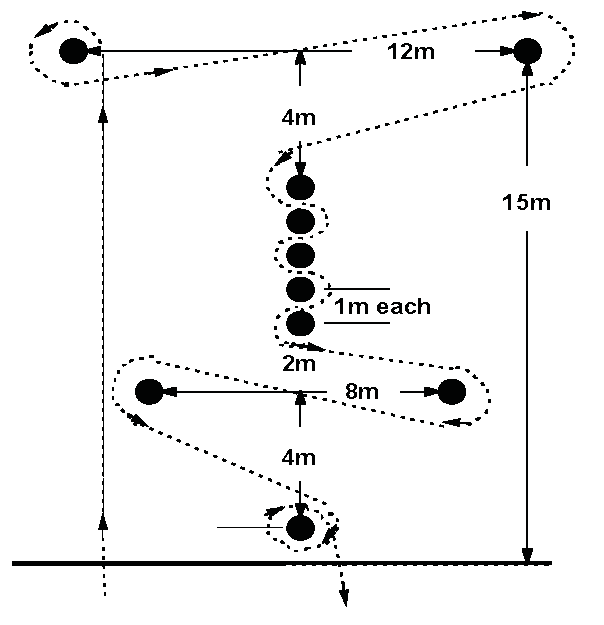
\includegraphics{iuf_slalom}
\end{center}
\vspace{-20pt}
\caption{IUF Slalom Course \label{fig:iuf_slalom}}
\vspace{-10pt}
\end{figure}
Pictured here is the IUF Slalom, in which you must ride around 10 cones in the correct pattern.
Arrows marked on the ground should indicate the direction of the turns for riders unfamiliar with the course.
The rider has to start directly behind the Start line.
The Starter gives the opening, and then the competitor has to start during the next 3 seconds.
The timer is started when any defined point of the tire (for example the part that crosses a low light beam) crosses the start line, and stops when a similar point of the tire crosses the finish line.
If the rider has not yet started after 3 seconds, the timer will start counting anyway.
The rider is not disqualified for this.
Time measurement at start and finish line must be identical to insure accurate time measurement.
It must be secured that riders do not gain momentum before crossing the start line (no flying starts).
Remounting is not allowed. 
Cones may be hit, but not knocked over.
vThe course must be followed correctly, including the direction of turns.
The last cone must be completely circled before the rider's time is taken at the finish line.
Riders who go the wrong way around a cone can go back and make the turn the correct way with the clock still running.
The cones used are plastic traffic cones.
For official competition, cones must be between 45 and 60 cm tall, with bases no more than 30 cm square.
The course must be set up accurately.
The proper positions of the cones should be marked on the ground for a cone to be replaced quickly after it has been knocked over.
Riders get two attempts.
